\documentclass[10pt,a4paper]{article}
\usepackage[margin=1.9cm]{geometry}
\usepackage[T1]{fontenc}
\usepackage{lmodern,microtype,graphicx,booktabs,longtable,tabularx,array,enumitem,float,amsmath,amssymb,makecell,multirow}
\usepackage[table]{xcolor}
\usepackage[most]{tcolorbox}
\usepackage[font=small,labelfont=bf]{caption}
\usepackage[colorlinks=true,linkcolor=blue!50!black,urlcolor=blue!50!black]{hyperref}
\setlist{nosep,leftmargin=1.2em}
\setlength{\parindent}{0pt}\setlength{\parskip}{4pt}

\newtcolorbox{rev}[1][Reviewer]{breakable,enhanced,colback=gray!7,colframe=gray!55,title={#1},fonttitle=\bfseries\small,fontupper=\small\itshape,left=4pt,right=4pt,top=2pt,bottom=2pt}
\newtcolorbox{todo}[1][What to do]{breakable,enhanced,colback=blue!3,colframe=blue!45!black,title={#1},fonttitle=\bfseries\small,fontupper=\small,left=4pt,right=4pt,top=2pt,bottom=2pt}
\newtcolorbox{resp}{breakable,enhanced,colback=green!3,colframe=green!35!black,title={Draft response},fonttitle=\bfseries\small,fontupper=\small,left=4pt,right=4pt,top=2pt,bottom=2pt}
\newtcolorbox{priv}[1][For you only (not for the reviewer)]{breakable,enhanced,colback=red!3,colframe=red!55!black,title={#1},fonttitle=\bfseries\small,fontupper=\small,left=4pt,right=4pt,top=2pt,bottom=2pt}
\newcommand{\FILL}[1]{\textcolor{orange!85!black}{\textbf{[FILL: #1]}}}
\newcommand{\vf}{\textsuperscript{\textcolor{orange!85!black}{\textbf{v}}}}
\newcommand{\fig}[2][\linewidth]{\begin{center}\includegraphics[width=#1]{#2}\end{center}}

\begin{document}
\begin{center}
{\LARGE\bfseries Manuscript AIS 3400076: revision workbook}\\[4pt]
{\large Every reviewer and editor comment, what to change, evidence, and draft responses}\\[4pt]
{\small Prepared from the revision letter (22 Sep 2026), the submitted manuscript and SI, the repository code and the original datasets. October 2026.}
\end{center}

\section*{How to read this document}
\begin{itemize}
\item \colorbox{gray!15}{Grey boxes}: the reviewer's or editor's words, verbatim.
\item \colorbox{blue!8}{Blue boxes}: what to change. By default changes are minimal; a figure is only modified when the reviewer asks for it, and the reason is given.
\item \colorbox{green!8}{Green boxes}: draft response text, ready to adapt for the response letter.
\item \colorbox{red!8}{Red boxes}: notes for you only. They describe things found in the code or data that you should know before submitting; they are not meant for the reviewer.
\item \FILL{...}: information that only you have (hardware details, decisions).
\item \vf\ in the comparison table: taken from abstracts or secondary sources; check against the full paper before submission.
\end{itemize}
\textbf{Ground rules used.} The paper is the reference: responses build on what it already states, and changes are only proposed where the reviewer asks for them. Agreed exceptions: the ``up to 85$^\circ$'' bending figure is replaced by the measured values; Comment 4 is answered with the ``model-constrained reconstruction'' framing.

\textbf{What was verified.} The published numbers below were reproduced from the repository and the original datasets (same models, same test split): Table~1 (to the decimal), Table~S6 (to the decimal), Fig.~5c, Fig.~8b, Table~2, the bar heights of Fig.~7a/7b, and Table~S5 (within 0.02\,mm / 0.08$^\circ$). The original 85/10/5 split is reproducible: every notebook sets \texttt{seed = 42} for \texttt{random}, NumPy and PyTorch in its first cell, and the split calls \texttt{train\_test\_split} without \texttt{random\_state}, i.e.\ from that seeded stream.

\subsection*{Overview of all comments}
\small
\begin{longtable}{p{0.8cm}p{6.4cm}p{6.3cm}p{1.6cm}}
\toprule
ID & Comment & Action & Section\\\midrule\endhead
E1 & Title precise and searchable & No change needed & \ref{sec:editor}\\
E2 & Suggested references (optional) & Add Hofer, Thuruthel, Han, Lu; Yoo is already Ref.~[15] & \ref{sec:comp}\\
E3 & Proofread, define acronyms & Acronym audit list & \ref{sec:editor}\\
E4 & Figure text and captions complete & Handled figure by figure & \ref{sec:figs}\\
E5 & Copyright of reused images & Statement & \ref{sec:editor}\\
E6 & Reference style, full titles, DOIs & Add DOIs & \ref{sec:editor}\\\midrule
R1 & Role of visual sensing in control & Text, Fig.~4c, Alg.~1 & \ref{sec:f4}, \ref{sec:ctrl}\\
R2 & Originality vs.\ prior work & Comparison table + paragraph & \ref{sec:comp}\\
R3 & Scalability claim & Narrow the wording & \ref{sec:claims}\\
R4 & Ground truth for full-body reconstruction & Model-constrained framing, assumptions, S2b details & \ref{sec:fs2}, \ref{sec:data}\\
R5 & Curvature-coordinate inconsistency & Use dimensional arc length (as code and SI) & \ref{sec:model}\\
R6 & Secondary objective not evaluated & Offline ablations (both controllers), reframe $H(l)$ & \ref{sec:results}\\
R7 & Control evaluation narrow & Coverage numbers, wording, limitations & \ref{sec:results}, \ref{sec:fs456}\\
R8 & Train/test independence & Split description, leakage analysis & \ref{sec:data}\\
R9 & Reproducibility details & SI table + \FILL{} items & \ref{sec:nets}, \ref{sec:hw}, App.~\ref{app:repro}\\
R10 & Figures 1B, 2, 3, 5 & Part 1 & \ref{sec:figs}\\\midrule
m1 & ``Markerless'' & ``markerless at inference'' & \ref{sec:claims}\\
m2 & Section vs.\ segment & Use ``section'' everywhere & \ref{sec:claims}\\
m3 & ``All ten tendons'' & Three (single) / nine (multi) & \ref{sec:hw}\\
m4 & Camera model, lens, FOV, rate, size & \FILL{} & \ref{sec:hw}\\
m5 & ``Simultaneous'' acquisition & Describe software synchronisation & \ref{sec:f1}, \ref{sec:hw}\\
m6 & Sine/cosine decoding, loss balance & No decoding needed; explain & \ref{sec:nets}\\
m7 & Sign in Eq.~S11, highlighted pixels & Explain; Fig.~4a caption & \ref{sec:f4}, \ref{sec:nets}\\
m8 & Unused PCC line in Alg.~1 & It sets the encoder offset; explain & \ref{sec:ctrl}\\
m9 & Jacobian notation & One consistent notation & \ref{sec:ctrl}\\
m10 & Open-loop baselines; terminology & Same planner/gains; ``open-loop'' & \ref{sec:ctrl}\\
m11 & Denominators of percentages & State them & \ref{sec:results}\\
m12 & Fig.~5b axis scaling & Equal scaling / scale bar & \ref{sec:f5}\\
m13 & Fig.~7 statistic & Per-point error vs.\ arc length & \ref{sec:f7}\\
m14 & Table~1 robust statistics & Median, p95, max & \ref{sec:results}\\
m15 & ``Bent configurations improve accuracy'' & Error vs.\ bending plot & \ref{sec:fnew}, \ref{sec:results}\\
m16 & Figs.~6, 9, 10 details, path errors & Captions + table & \ref{sec:f6}\\
m17 & Discussion: demonstrated vs.\ proposed & Rewrite & \ref{sec:claims}\\\midrule
S1 & Fig.~S2b numbers & Caption + numbers & \ref{sec:fs2}\\
S2 & Table~S6 skewed errors & Robust stats + outliers & \ref{sec:results}\\
S3 & Figs.~S4--S6 matched IDs, colours & Regenerated & \ref{sec:fs456}\\
S4 & Tables~S3/S4 composition & Dataset composition text & \ref{sec:data}\\
\bottomrule
\end{longtable}
\normalsize

%==========================================================================
\clearpage
\part*{Part 1 --- Figures and captions}\addcontentsline{toc}{part}{Part 1}
\label{sec:figs}
\setcounter{section}{1}\setcounter{subsection}{0}
\renewcommand{\thesubsection}{1.\arabic{subsection}}

\begin{rev}[Reviewer, Comment 10]
Several figures---particularly Figs.~1B, 2, 3, and 5---are difficult to interpret. Their visual density and inconsistent presentation make it hard to follow the methodology and compare results. In particular, Figure~3 requires attention. [\dots] The paper should use a consistent flow direction, label all network inputs and outputs, and distinguish clearly between the networks used for pose estimation, curvature reconstruction, forward kinematics, and inverse kinematics.
\end{rev}

\textbf{Summary of figure changes.} Only Fig.~3, Fig.~7 and Figs.~S4--S6 need a real redraw; Fig.~4c and Fig.~5b need one small addition each; everything else is caption wording.

\small
\begin{tabularx}{\linewidth}{lXl}
\toprule
Figure & Change & Type\\\midrule
1 & ``simultaneously'' $\rightarrow$ synchronisation wording; ``segments'' $\rightarrow$ ``sections'' & caption\\
2 & One sentence explaining $L_1$--$L_4$ vs.\ tendons $\delta_i$ & caption\\
3 & Label every network, its inputs/outputs and tensor sizes; one flow direction & redraw\\
4a & Define what the colour map shows & caption\\
4c & Add the encoder branch (model-based only) and mark curvature as outside the loop & small edit\\
5b & Equal axis scaling or add scale bar & small edit\\
5c, 8b & ``section''; define CL/OL; error bars are across targets & caption\\
6, 9, 10 & Start point, direction, cycles, single run, ``open-loop''; path errors & caption + table\\
7 & Per-point error vs.\ normalised arc length; define statistic & redraw\\
S1 & ``multi-segment'' $\rightarrow$ ``multi-section'' & caption\\
S2 & Interval type, $N$, independence & caption\\
S3 & Jacobian symbols as in main text & small edit\\
S4--S6 & Matched target IDs, shared colour limits & redraw\\
New (SI) & Error vs.\ bending angle; null-space ablation & new\\
\bottomrule
\end{tabularx}
\normalsize

%--------------------------------------------------------------------------
\subsection{Figure 1}\label{sec:f1}
\fig[0.9\linewidth]{../crops/fig1_annot.png}
\begin{rev}[Reviewer, minor pp.~1--2 and 3--5]
Use either `section' or `segment' consistently throughout the manuscript, figures, algorithms, and SI. [\dots] The claim that images are acquired simultaneously should be supported by the synchronization method as this type software capture is not necessarily simultaneous hardware triggering.
\end{rev}
\begin{todo}
Caption only. The cameras are read by one capture thread each, with no shared trigger (\texttt{MULTI\_cameras\_utility.py}: each thread keeps the latest frame; the controller reads the three latest frames). Fig.~1B: reviewer's comment is generic; keep the content, at most enlarge the panel labels.

Proposed caption: ``(a) Multi-section soft robot arm sensorisation and reconstruction pipeline. Images from the three cameras are read concurrently by software (one capture thread per camera, latest frame used; no hardware trigger) and fed to CNNs, which predict both the tip poses and the full-body curvature. (b) Robot setup. The tendon-driven arm consists of three independent \emph{sections}, each actuated by three motors, with Bowden cables routing the tendons of sections II and III. The optical tracking system provides the ground-truth configuration.''
\end{todo}

\subsection{Figure 2}
\fig[0.6\linewidth]{../crops/fig2_annot.png}
\begin{todo}
Caption only (R10 lists Fig.~2 as dense, without a specific request). The source of confusion is that four boundary arcs $L_1$--$L_4$ are drawn next to three tendons $\delta_1$--$\delta_3$. Add: ``$L_1$--$L_4$ are the arcs at distance $d$ from the axis along $\pm x$ and $\pm y$ that define $\Delta_x$ and $\Delta_y$ (Eq.~S2); they are geometric constructions, not tendons. The three tendons are placed at angles $\delta_i$ on the same circle (left).''
\end{todo}

\subsection{Figure 3}
\fig[0.95\linewidth]{../crops/fig3_annot.png}
\begin{todo}[What to do (redraw, requested explicitly)]
Keep the two panels, but (i) use left-to-right flow throughout, (ii) write the network name on each path ($f_p^1$, $f_p^3$, $f_C^1$, $f_C^3$, $N_l^1$, $N_p^3$, $N_l^3$, $N_C$), (iii) annotate the tensor sizes and outputs, (iv) colour by role (pose / curvature / forward kinematics / inverse kinematics). The proposed map below is generated from the code and can be used as panel (c) or as the template:
\fig[0.95\linewidth]{../figures/network_map.pdf}
Facts from the code that the figure must show (marker \textcircled{\small 1}, \textcircled{\small 2}):
\begin{itemize}
\item Single-section: the first convolution of MobileNetV2 is replaced by a 1-channel one; head \texttt{Linear(1280$\to$6)} for $f_p^1$ and \texttt{Linear(1280$\to$5|4|3)} for $f_C^1$.
\item Multi-section: the three grayscale images are the three input channels of the pretrained 3-channel convolution; heads are two layers, \texttt{1280$\to$512$\to$18} for $f_p^3$ and \texttt{1280$\to$512$\to$15|12|9} for $f_C^3$. The current figure shows a single ``Linear Layer'' for all heads.
\item Panel (b) (residual MLP with BatchNorm and LeakyReLU, 3 residual blocks of width 128) describes $N_l^1$ and $N_C$. The multi-section kinematic networks $N_p^3$ (9$\to$6) and $N_l^3$ (6$\to$9) are plain MLPs with four hidden layers of 128 units and ELU activations. Either show both or state this in the caption.
\end{itemize}
Caption addition: ``Inputs and outputs: $f_p^n$: $n\times480\times640$ images $\to$ section-tip poses ($6n$); $f_C^n$: images $\to$ curvature parameters per section (5/4/3 for quadratic/affine/constant); $N_l^1$: tip position (3) $\to$ tendon lengths (3); $N_p^3$: tendon lengths (9) $\to$ tip pose (6); $N_l^3$: tip pose (6) $\to$ tendon lengths (9), trained through the frozen $N_p^3$; $N_C$: section-tip pose in the section frame (6) $\to$ curvature parameters of that section (used offline to label the multi-section dataset).''
\end{todo}
\begin{resp}
We thank the reviewer. Figure~3 has been redrawn with a single left-to-right flow, the name of each network on its path, the input and output of every network with tensor dimensions, and colours that separate pose estimation, curvature reconstruction, forward kinematics and inverse kinematics. The caption now lists the inputs and outputs of all networks, and states which architecture is used for the single- and multi-section kinematic networks.
\end{resp}

\subsection{Figure 4}\label{sec:f4}
\fig[0.95\linewidth]{../crops/fig4_annot.png}
\begin{rev}[Reviewer, Comment 1 (excerpt) and minor pp.~5--7]
The abstract, contribution list, Fig.~4c, and conclusion should clearly distinguish: camera-based pose estimation used for control; encoder measurements used to calculate the Jacobian and null-space term; and image-based PPC reconstruction evaluated as a separate sensing capability. [\dots] Clarify the negative sign in Eq.~S11 and clarify how the highlighted pixels are the regions used for prediction.
\end{rev}
\begin{todo}
\textbf{4c} (marker \textcircled{\small 2}): one added block and one arrow. Encoders read $l$ and feed $J(l)$ and $N(\bar l-l)$ in the model-based branch only; the curvature CNN is drawn as an output that does not enter the loop. Proposed:
\fig[0.95\linewidth]{../figures/fig4c_proposed.pdf}
Caption addition: ``Camera images provide the tip pose $p$ used in the error $p_\text{ref}-p$ for both controllers. In the model-based controller, motor encoders provide $l$ for the PCC Jacobian and the null-space term; the data-driven controller does not use encoders. The curvature reconstruction $f_C$ is a separate output and does not enter either control law.''

\textbf{4a} (marker \textcircled{\small 1}): caption addition: ``Colours show the Grad-CAM map of the last convolutional layer for the target $-\mathcal{L}$ (negative loss), passed through ReLU and normalised to [0,1] per image; warm colours mark regions whose activation most reduces the prediction loss. No threshold is applied. The last panel is the mean map over the test set.''
\end{todo}

\subsection{Figure 5}\label{sec:f5}
\fig[0.95\linewidth]{../crops/fig5_annot.png}
\begin{rev}[Reviewer, minor pp.~8--11]
Figure~5b intentionally uses nonuniform axis scaling. This visually distorts the reconstructed shapes. Use equal spatial scaling where possible or add a second undistorted view and explicit scale bars.
\end{rev}
\begin{todo}
\textbf{5b} (marker \textcircled{\small 1}): use equal axis scaling in the shape panels and add a 20\,mm scale bar; the curves stay readable (example generated with the same models and four test configurations of increasing bending):
\fig[0.75\linewidth]{../figures/fig5b_proposed.pdf}
Remove ``Axes scaling is not uniform to emphasize the bending effect'' from the caption and add ``Axes have equal scaling; scale bar 20\,mm.''

\textbf{5c} caption: ``single-segment'' $\rightarrow$ ``single-section''; add ``CL: closed-loop, OL: open-loop. Bars: mean over the 20 targets; error bars: one standard deviation across targets (each target visited once), not trial-to-trial repeatability.''
\end{todo}
\begin{resp}
We agree that the non-uniform scaling distorted the shapes. The shape panels of Fig.~5b now use equal axis scaling and a scale bar, and the caption no longer refers to non-uniform scaling.
\end{resp}

\subsection{Figures 6, 9 and 10}\label{sec:f6}
\fig[0.9\linewidth]{../crops/fig6_annot.png}
\fig[0.9\linewidth]{../crops/fig9_annot.png}
\fig[0.75\linewidth]{../crops/fig10_annot.png}
\begin{rev}[Reviewer, minor pp.~5--7 and 8--11]
`Open-loop' and `feedforward' should be used consistently. [\dots] For Figs.~6, 9, and 10, identify the start direction, waypoint order, number of completed cycles, and whether the plotted paths are one run or an average. Add quantitative path errors in the caption or an accompanying table.
\end{rev}
\begin{todo}
Captions only, plus one table (below). From the logged trajectories and \texttt{generate\_polygon\_vertices}: every path starts at angle $0$ (point $(+r,0)$), follows the 30 vertices counter-clockwise, completes one cycle, and each plotted path is a single run (no averaging). The panels already say ``open-loop''; replace ``feedforward'' in the captions. In Figs.~9 and 10, ``Angular values'' $\rightarrow$ ``mean $\pm$ std orientation error along each circle''.

Caption sentence: ``Each path is a single run of one cycle, starting at $(x,y)=(r,0)$ and traversing the 30 waypoints counter-clockwise. Path errors are given in Table~S\,X.''

\textbf{Path errors} (radial RMS = RMS of the distance from the reference circle; height RMS = RMS of $z-z_\text{ref}$; circle centre and radius fitted to the commanded vertices of each run):
\begin{center}\small
\begin{tabular}{lllrrrrr}
\toprule
Arm & Controller & Loop & $r$ [mm] & $z$ [mm] & Radial RMS [mm] & Height RMS [mm] & samples\\\midrule
Single & Data-driven & closed & 34.6 & 115 & 1.71 & 2.49 & 2923 \\
Single & Model-based & closed & 31.4 & 115 & 1.46 & 2.65 & 2991 \\
Single & Data-driven & closed & 24.9 & 125 & 1.83 & 1.54 & 2040 \\
Single & Model-based & closed & 22.4 & 125 & 1.32 & 1.23 & 2083 \\
Single & Data-driven & open & 34.6 & 115 & 2.27 & 5.48 & 3259 \\
Single & Model-based & open & 31.4 & 115 & 8.06 & 8.74 & 3401 \\
Single & Data-driven & open & 24.9 & 125 & 1.61 & 4.41 & 2289 \\
Single & Model-based & open & 22.4 & 125 & 5.71 & 4.30 & 2450 \\
Multi & Data-driven & closed & 120.0 & 350 & 7.63 & 2.10 & 19847 \\
Multi & Data-driven & closed & 80.0 & 380 & 5.85 & 2.72 & 17218 \\
Multi & Model-based & closed & 120.0 & 350 & 7.78 & 5.74 & 43240 \\
Multi & Model-based & closed & 80.0 & 380 & 6.25 & 3.43 & 19847 \\
Multi & Model-based + 50 g & closed & 120.0 & 350 & 11.46 & 6.46 & 20000 \\
Multi & Model-based + 50 g & closed & 80.0 & 380 & 5.35 & 1.63 & 20000 \\
Multi & Data-driven & open & 120.0 & 350 & 10.86 & 4.41 & 1818 \\
Multi & Data-driven & open & 80.0 & 380 & 5.53 & 7.67 & 1208 \\
Multi & Model-based & open & 120.0 & 350 & 12.64 & 8.10 & 1835 \\
Multi & Model-based & open & 80.0 & 380 & 10.60 & 5.24 & 1213 \\
Multi & Model-based + 50 g & open & 120.0 & 350 & 27.10 & 28.46 & 1824 \\
Multi & Model-based + 50 g & open & 80.0 & 380 & 20.64 & 11.22 & 1218 \\
\bottomrule
\end{tabular}
\end{center}
\end{todo}
\begin{resp}
We now use ``open-loop'' throughout. The captions of Figs.~6, 9 and 10 state that each path is a single run of one counter-clockwise cycle starting at $(r,0)$, and a new table (Table~S\,X) reports the radial and height RMS deviation from the reference circle for every controller, arm and load condition. For example, under the 50\,g payload the radial RMS error on the 120\,mm circle is 11.5\,mm in closed loop and 27.1\,mm in open loop.
\end{resp}

\subsection{Figure 7}\label{sec:f7}
\fig[0.55\linewidth]{../crops/fig7_annot.png}
\begin{rev}[Reviewer, minor pp.~8--11]
Figure~7 alternates among `cumulative 3D error,' `sum of 3D errors,' and `average 3D error for each point.' Define the statistic exactly. Summing three points for the single-section arm and nine for the multi-section arm also prevents direct comparison. Per-point RMSE or error versus normalized arc length would be clearer.
\end{rev}
\begin{todo}[What to do (redraw, requested explicitly)]
Replace the stacked bars by the per-point error against normalised arc length, same models, same test set (the bar heights of the current figure are reproduced: 7.8/7.9/8.3\,mm and 209/203/198\,mm). Points: median; whiskers: interquartile range.
\fig[0.95\linewidth]{../figures/fig7_proposed.pdf}
Per-point RMSE (mm), for the table or caption:\\[2pt]
\small
\begin{tabular}{llll}
\toprule
Model & Single ($L/3,\ 2L/3,\ L$) & Multi, 9 points (base $\to$ tip)\\\midrule
Constant & 0.82, 2.95, 6.46 & 1.3, 5.1, 11.3, 18.9, 27.3, 37.0, 48.0, 59.8, 72.4\\
Affine & 0.84, 2.94, 6.33 & 1.3, 5.1, 11.3, 18.9, 27.4, 37.0, 47.8, 59.4, 71.7\\
Quadratic & 0.90, 3.21, 6.98 & 1.2, 4.9, 11.0, 18.2, 25.9, 34.9, 45.2, 56.2, 68.1\\
\bottomrule
\end{tabular}\normalsize

Caption: ``3D reconstruction error of the curvature models at points along the backbone, as a function of the normalised arc length from the base. For each test sample, the backbone reconstructed from the predicted curvature parameters is compared with the one reconstructed from the labels at $s/L=1/3,2/3,1$ (single section) and at every ninth of the arm (multi-section). Markers: median over the test set ($N=500$); whiskers: interquartile range. Multi-section labels are model-constrained (Section~2.2).''
\end{todo}
\begin{resp}
We agree that the summed statistic was ambiguous and not comparable between the two arms. Figure~7 now shows the 3D error at each reference point against the normalised arc length, for both arms on the same horizontal axis (median and interquartile range over the 500 test samples), and the caption defines the statistic. The per-point RMSE values are also reported.
\end{resp}

\subsection{Figure 8}
\fig[0.85\linewidth]{../crops/fig8_annot.png}
\begin{todo}
Caption only: ``multi-segment'' $\rightarrow$ ``multi-section''; define CL/OL; ``error bars: one standard deviation across the 20 targets (each visited once)''.
\end{todo}

\subsection{Figure S1}
\fig[0.6\linewidth]{../crops/figS1_annot.png}
\begin{todo}
Caption: ``Workspace of the multi-section robot. Sampled positions of the first, second and third section tips [\dots]''.
\end{todo}

\subsection{Figure S2}\label{sec:fs2}
\fig[0.6\linewidth]{../crops/figS2_annot.png}
\begin{rev}[Reviewer, Comment 4 (excerpt) and SI comment]
Fig.~S2b does not provide sufficient validation of N\_C: numerical errors, sample count, data split, and confidence intervals are missing. It is also unclear whether its validation configurations are independent of the data used to train N\_C and the three-section curvature estimator. [\dots] Fig.~S2b should report the numerical N\_C error for each curvature model, the number of validation configurations, and whether the bars show standard deviation, standard error, or another interval.
\end{rev}
\begin{todo}
Caption additions for S2b, all from the code (\texttt{MULTI\_curvature\_checks.py}, testing notebook):
\begin{itemize}
\item Number of validation configurations: \textbf{20}, posed manually with every backbone marker visible, recorded in a separate session.
\item Bars: sum over the nine reference points of the mean per-point error; whiskers: \textbf{one standard deviation} (sample, ddof\,=\,1) of the per-configuration sum across the 20 configurations.
\item Independence: $N_C$ was trained on the single-section dataset only; the 20 configurations are not part of its training data nor of the multi-section CNN training data.
\item $N_C$ error on held-out data of its own domain (single-section test split, $N=500$, never used for training), 3D error at $L/3$, $2L/3$, $L$: constant 0.38/1.20/2.49\,mm, affine 0.42/1.35/2.76\,mm, quadratic 0.43/1.37/2.94\,mm (sums $4.1\pm4.8$, $4.5\pm5.6$, $4.7\pm6.0$\,mm).
\end{itemize}
S2a is the same data as Fig.~7b; once Fig.~7 is redrawn, either remove S2a or redraw it in the same per-point form.
\end{todo}
\begin{priv}
See note~\ref{priv:s2b} at the end of Part~3 before finalising anything that cites S2b values.
\end{priv}

\subsection{Figure S3}
\fig[0.9\linewidth]{../crops/figS3_annot.png}
\begin{todo}
Only the symbols: use the same Jacobian notation as the main text (Section~\ref{sec:ctrl}), e.g.\ $J_{l\to p}(l)$ for the PCC Jacobian and $\hat J_{p\to l}$ for the learned one.
\end{todo}

\subsection{Figures S4--S6}\label{sec:fs456}
\begin{minipage}{0.48\linewidth}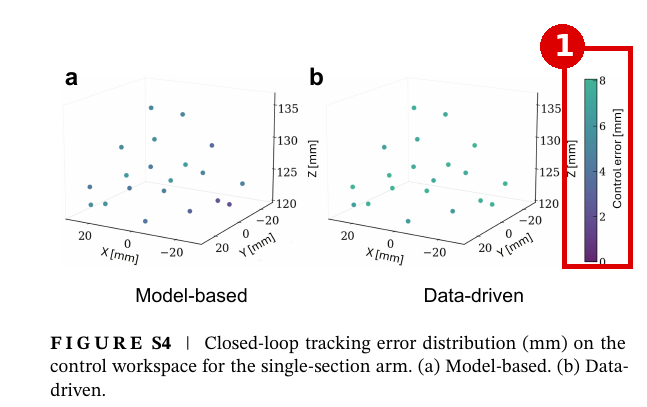
\includegraphics[width=\linewidth]{../crops/figS4_annot.png}\end{minipage}\hfill
\begin{minipage}{0.48\linewidth}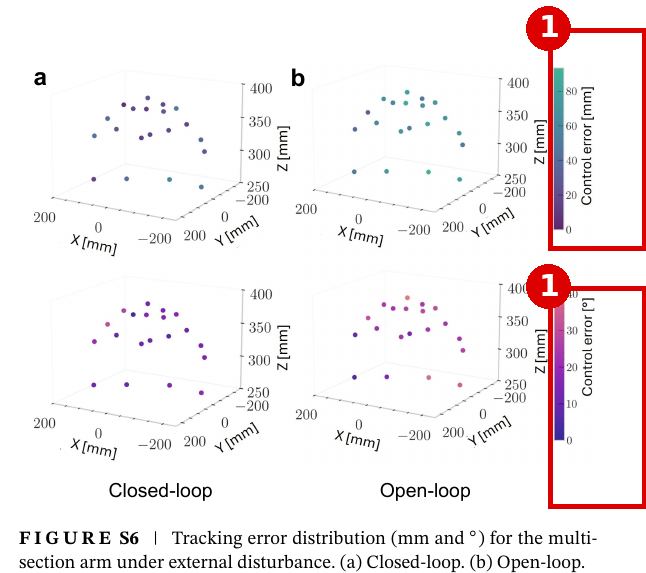
\includegraphics[width=\linewidth]{../crops/figS6_annot.png}\end{minipage}
\begin{rev}[Reviewer, SI comment and Comment 7 (excerpt)]
Figs.~S4--S6 should use matched target identifiers or connecting pairs so the reader can compare the same workspace locations across controllers. Use consistent color limits when the goal is direct visual comparison. [\dots] the coordinates are not tabulated and the targets are not compared with the complete reachable or sampled workspace.
\end{rev}
\begin{todo}[What to do (redraw, requested explicitly)]
Same plots, two changes: every target carries its ID (1--20, same as the coordinate tables in App.~\ref{app:targets}), and each figure uses one colour scale per quantity (marker \textcircled{\small 1} shows the current independent colour bars).
\fig[0.75\linewidth]{../figures/figS4_proposed.pdf}
\fig[0.8\linewidth]{../figures/figS5_proposed.pdf}
\fig[0.8\linewidth]{../figures/figS6_proposed.pdf}
Add the target coordinate tables (App.~\ref{app:targets}) to the SI, and the coverage statement of Section~\ref{sec:results} (R7).
\end{todo}
\begin{resp}
Figures~S4--S6 now label each of the 20 targets with the same identifier in every panel, and use a single colour scale per quantity within each figure. The target coordinates, with the bending angle and length change of each section, are tabulated in the SI (Tables~S\,Y and S\,Z).
\end{resp}

\subsection{New SI figures}\label{sec:fnew}
\textbf{Error vs.\ bending angle} (minor pp.~8--11, ``The authors should plot error against bending angle before drawing this conclusion''):
\fig[0.98\linewidth]{../figures/bending_error.pdf}
Bending angle of the single section from the tip orientation label; for the multi-section arm, bending of each section from the relative orientation of consecutive tips. Black: binned median, band: interquartile range. See Section~\ref{sec:results} for the wording this supports.

\textbf{Null-space ablation} (R6), already in the repository (\texttt{MULTI\_nullspace\_ablation.ipynb}):
\fig[0.8\linewidth]{../figures/repo_nullspace_ablation.pdf}

%==========================================================================
\clearpage
\part*{Part 2 --- Comparison with prior work (Comment 2)}\addcontentsline{toc}{part}{Part 2}
\setcounter{section}{2}\setcounter{subsection}{0}
\renewcommand{\thesubsection}{2.\arabic{subsection}}
\label{sec:comp}
\begin{rev}[Reviewer, Comment 2]
The individual sensing and control elements of this paper have appeared in many papers. [\dots] Several particularly relevant studies are missing or insufficiently discussed: Hofer et al.\ (2021) [\dots] Thuruthel et al.\ (2017) [\dots] Han et al.\ (2025) [\dots] Lu et al.\ (2024) [\dots] Yoo et al.\ [\dots] The authors should explain what each close prior study established and identify the specific capability added here. The claim that no prior framework combines comparable sensing with closed-loop null-space control is too broad without this analysis.
\end{rev}

\subsection{Comparison table}
\scriptsize
\begin{longtable}{p{1.6cm}p{2.3cm}p{2.0cm}p{0.9cm}p{2.2cm}p{2.0cm}p{1.7cm}p{1.5cm}p{1.6cm}}
\toprule
Work & Sensing & Robot / actuation & Sect. & Estimated & Closed loop on estimate & Redundancy used & Load / disturbance & Accuracy, rate\\\midrule\endhead
Hofer et al.\ 2021 & 3 internal cameras (one per bellow), painted interior pattern, LED illumination & Pneumatic fabric spherical arm, 3 bellows, 2 rotational DoF & 1 & Orientation (2 angles) & Yes: cascaded PI on camera orientation & No (redundant in pressure, not exploited) & Not tested (future work) & $\approx$1$^\circ$ RMS, 30\,Hz\\
Thuruthel et al.\ 2017 & External tip sensing (electromagnetic\vf) & Redundant continuum manipulator (tendon-driven per reviewer\vf) & multi\vf & Tip position & Yes: learned IK with end-effector feedback & Implicit in learned IK; no explicit secondary objective\vf & External loads (per reviewer) & \vf\\
Han et al.\ 2025 & 1 internal camera tracking an anchor marker & Metastructure modules (ProSoRo); tendon-driven platform in demos & per module & Anchor 6-DoF motion, 6-axis force, full-body shape (FEA-trained MVAE) & Not demonstrated & --- & Contact tasks; force vs.\ F/T sensor & not on project page\vf\\
Lu et al.\ 2024 & Multi-core FBG (not vision) & Colonoscope and multi-section extensible soft manipulators & multi & 3-D shape & Yes: adaptive online-learning shape servoing & Not mentioned\vf & Unstructured environments, disturbances & \vf\\
Yoo et al.\ 2023 (Ref.~15) & Internal camera, sim-to-real (zero-shot) & Pneumatic soft actuator & 1 & 3-D shape & No & --- & --- & \vf\\
\rowcolor{blue!6}This work & One internal camera per section, no internal markers or patterns; mocap only for labels & Tendon-driven Trimmed Helicoid, 3 motors per section & 1 and 3 & Section-tip 6-DoF poses + PPC curvature per section & Yes: model-based (PCC Jacobian) and data-driven (learned IK) on camera pose & Yes: null-space objective (model-based) and Lagrangian term in IK training (data-driven) & 50\,g tip payload (one condition) & Single: 3.99\,mm/3.11$^\circ$ (static); multi tip: 26.45\,mm; $\approx$8\,Hz\\
\bottomrule
\end{longtable}
\normalsize
Sources: Hofer et al.\ from the full text (Frontiers); Han et al.\ from the project page (\url{https://prosoro.github.io}); Thuruthel et al.\ and Lu et al.\ from abstracts and citing works (the full texts were not accessible); Yoo et al.\ is already cited in the manuscript. Cells marked \vf\ must be checked against the full paper.

\subsection{Text for the Introduction}
\begin{todo}
Insert after the sentence ending ``\dots closed-loop null-space control of continuum robots, either through model-based or learning-based approaches.'' and narrow the novelty claim accordingly. Draft:

``Several systems combine embedded sensing with closed-loop control of soft or continuum arms. Hofer et al.\ placed one camera inside each of the three fabric bellows of a pneumatic spherical arm, observed a painted interior pattern, and regulated the two joint angles in closed loop with about 1$^\circ$ accuracy at 30\,Hz; the arm is redundant in actuation, but this redundancy was not exploited [H]. Thuruthel et al.\ learned inverse kinematics with end-effector feedback for a redundant continuum manipulator, including operation under external loads [T]. Han et al.\ tracked an internal anchor marker with a single onboard camera to infer the full-body deformation and contact force of a soft module [Ha], and Yoo et al.\ estimated the 3-D shape of a pneumatic actuator from an internal camera with a model trained in simulation [15]; neither closed a control loop on the estimate. Lu et al.\ servoed the 3-D shape of continuum and soft robots in unstructured environments with adaptive online learning, using fibre Bragg grating rather than visual sensing [L]. The present work differs in two respects: it distributes one internal camera per section along a multi-section tendon-driven arm, without internal markers, patterns or dedicated illumination, and it closes the loop on the camera-estimated pose with controllers that resolve the actuation redundancy explicitly, either in the null space of a model-based Jacobian or through a secondary objective in the training of a learned inverse kinematics. To our knowledge this combination has not been reported.''

Contribution list, item 1--2: state the integration claim precisely (``distributed internal cameras on a multi-section arm, markerless at inference, with redundancy-aware closed-loop control, model-based and learned'').
\end{todo}
\begin{resp}
We thank the reviewer for these references. We added Hofer et al., Thuruthel et al., Han et al.\ and Lu et al.\ (Yoo et al.\ was already cited as Ref.~[15]) and a paragraph in the Introduction that states what each study established. Hofer et al.\ obtain a higher orientation accuracy (about 1$^\circ$ at 30\,Hz) than our single-section estimate (3.11$^\circ$ at about 8\,Hz), on a two-angle spherical joint with an internal painted pattern and illumination; our system estimates the full 6-DoF tip pose of an extensible section without internal markers and scales to three sections. The capability we add is the combination of distributed internal cameras on a multi-section arm with closed-loop control that explicitly exploits the actuation redundancy (model-based null-space control and a learned inverse kinematics with a secondary objective). We have narrowed the novelty statement in the Introduction and in the contribution list to this combination, and a comparison table is provided in the SI.
\end{resp}

\textbf{New references} (BibTeX, matching your library's style):
{\scriptsize
\begin{verbatim}
@article{hoferVisionBasedSensingApproach2021,
  title = {A {{Vision-Based Sensing Approach}} for a {{Spherical Soft Robotic Arm}}},
  author = {Hofer, Matthias and Sferrazza, Carmelo and D'Andrea, Raffaello},
  year = 2021, journal = {Frontiers in Robotics and AI}, volume = {8}, pages = {630935},
  doi = {10.3389/frobt.2021.630935}}
@article{thuruthelLearningClosedLoop2017,
  title = {Learning {{Closed Loop Kinematic Controllers}} for {{Continuum Manipulators}} in {{Unstructured Environments}}},
  author = {Thuruthel, Thomas George and Falotico, Egidio and Manti, Mariangela and Pratesi, Andrea and Cianchetti, Matteo and Laschi, Cecilia},
  year = 2017, journal = {Soft Robotics}, volume = {4}, number = {3}, pages = {285--296},
  doi = {10.1089/soro.2016.0051}}
@article{hanAnchoringMorphologicalRepresentations2025,
  title = {Anchoring {{Morphological Representations Unlocks Latent Proprioception}} in {{Soft Robots}}},
  author = {Han, Xudong and Guo, Ning and Xu, Ruoyu and Wan, Fang and Song, Chaoyang},
  year = 2025, journal = {Advanced Intelligent Systems}, volume = {7}, number = {12}, pages = {e202500444},
  doi = {10.1002/aisy.202500444}}
@article{luAdaptiveOnlineLearning2024,
  title = {Adaptive {{Online Learning}} and {{Robust}} 3-{{D Shape Servoing}} of {{Continuum}} and {{Soft Robots}} in {{Unstructured Environments}}},
  author = {Lu, Yiang and Chen, Wei and Lu, Bo and Zhou, Jianshu and Chen, Zhi and Dou, Qi and Liu, Yun-Hui},
  year = 2024, journal = {Soft Robotics}, volume = {11}, number = {2}, pages = {320--337},
  doi = {10.1089/soro.2022.0158}}
\end{verbatim}}

%==========================================================================
\clearpage
\part*{Part 3 --- Everything else, by topic}\addcontentsline{toc}{part}{Part 3}
\setcounter{section}{3}\setcounter{subsection}{0}
\renewcommand{\thesubsection}{3.\arabic{subsection}}

\subsection{Editor's requirements}\label{sec:editor}
\begin{rev}[Editor]
Title succinct, descriptive and accurate [\dots] Reviewers may have suggested references [\dots] no obligation [\dots] define all acronyms when first mentioned (the title, abstract, and Table of Contents text must each be understandable as standalone texts). Check that the text and axis labels in all graphics are correct [\dots] all parts, insets, and footnotes of Figures [\dots] are mentioned in the caption. [\dots] copyright permission [\dots] full article titles, and optionally, DOIs.
\end{rev}
\begin{todo}
\begin{itemize}
\item \textbf{Title}: keep (states method, sensing and system).
\item \textbf{Suggested references}: all five addressed (Part~2); no need to decline any.
\item \textbf{Acronyms} to define at first use (and again in the abstract/ToC text if used there): PCC, PPC, CNN, MLP, GAP, IK, FK, SLERP, RRT, FBG, IMU, TPU, PLA, CL, OL, MVAE (if Han is described), Grad-CAM, SE(3)/SO(3). In figures: BW, FE, FC (Fig.~1a), BN1d (Fig.~3b), CL/OL (Figs.~5c, 8b).
\item \textbf{Figure text}: Part~1; every panel letter must appear in its caption (Fig.~1, 4, 5, 8 checked).
\item \textbf{Copyright}: all figures are original; state ``All figures were created by the authors for this manuscript.''
\item \textbf{References}: full titles are present; add DOIs (the four new ones are above).
\end{itemize}
\end{todo}

\subsection{Contribution, scope and claims}\label{sec:claims}
\begin{rev}[Reviewer, Comment 3]
The estimator is not invariant to the number of arm sections. [\dots] The output head must also change [\dots] Separate networks are trained for the one- and three-section arms. Transfer learning may reduce retraining effort, but the present method is not plug-and-play across arbitrary arm lengths and is not validated on an unseen section count. The statement that only the first layer must be adjusted also conflicts with Fig.~3 because the regression head changes as well.
\end{rev}
\begin{todo}
Text only. Section~3.1: replace ``adapting to a different number of sections requires adjusting only the first layer'' with ``adapting to a different number of sections requires changing the input layer (number of stacked camera channels) and the regression head (number of outputs), and retraining with the backbone transferred from the single-section network; we validated $n=1$ and $n=3$.'' Contribution~1: ``and can be extended to arms with a different number of sections by retraining with a transferred backbone''. Remove ``scalable'' where it implies no retraining (Abstract, Section~5 first sentence).
\end{todo}
\begin{resp}
We agree. The input layer and the regression head both depend on the number of sections, and separate networks were trained for the one- and three-section arms. We corrected the statement in Section~3.1, rephrased the contribution list and the Conclusion accordingly (the backbone is transferred, the network is retrained), and now state explicitly that only $n=1$ and $n=3$ were validated.
\end{resp}

\begin{rev}[Reviewer, minor pp.~1--2]
Use `markerless at measured inferences' rather than simply `markerless.' [\dots] Use either `section' or `segment' consistently throughout the manuscript, figures, algorithms, and SI.
\end{rev}
\begin{todo}
``markerless'' $\rightarrow$ ``markerless at inference (external motion-capture markers are used only to generate training labels)'' at first use, then ``markerless at inference''. Replace every ``segment'' by ``section''; occurrences: Main text: p.\,2 (2), p.\,3 (2), p.\,5 (4), p.\,6 (2), p.\,7 (1), p.\,8 (1), p.\,9 (4), p.\,11 (1). SI: p.\,1 (2), p.\,2 (4), p.\,3 (2), p.\,4 (3). This includes the headings of Sections~4.1 and 4.2 and the captions of Figs.~1, 5, 8 and S1.
\end{todo}
\begin{resp}
We now write ``markerless at inference'' and explain at first use that external motion-capture markers are only used to generate the training labels. We use ``section'' throughout the manuscript, figures, algorithms and SI.
\end{resp}

\begin{rev}[Reviewer, minor pp.~8--11 and Comment 9 (last sentence)]
The discussion should distinguish demonstrated capabilities from proposed applications. Obstacle avoidance, whole-body grasping, surgical guidance, and force or contact sensing are future directions and were not evaluated here. [\dots] Claims of robustness to lighting or hardware variation should be limited unless such variation was explicitly tested.
\end{rev}
\begin{todo}
Section~5: split into ``What was demonstrated'' (pose and curvature estimation from internal cameras; closed-loop pose control with two redundancy-aware controllers; one 50\,g payload condition) and ``Future directions'' (obstacle avoidance, whole-body grasping, surgical/inspection use, contact and force sensing). Remove or qualify ``variability is mitigated through image augmentations'' as a robustness claim: augmentations were used in training, robustness to lighting changes was not tested.
\end{todo}
\begin{resp}
We revised Section~5 to separate the capabilities evaluated in this work from future applications, which are now presented explicitly as future directions. We also removed the implication that the system is robust to lighting or hardware changes: image augmentations were used during training, but such variations were not tested.
\end{resp}

\subsection{How sensing enters the control loop}\label{sec:ctrl}
\begin{rev}[Reviewer, Comment 1]
[\dots] Algorithms~1 and 2 and Fig.~S3 indicate that both controllers use feedback from the pose network, while the curvature network is evaluated separately and does not enter either control law. Algorithm~1 also uses a PCC inverse calculation to initialize tendon lengths from section-tip positions. [\dots] the resulting estimate appears to be replaced by the motor-encoder measurement at the first control iteration, before it affects the control command. The authors should explain this initialization or remove it. The abstract, contribution list, Fig.~4c, and conclusion should clearly distinguish [\dots]
\end{rev}
\fig[0.48\linewidth]{../crops/alg1_annot.png}
\begin{todo}
The line is not discarded. In the code (\texttt{MULTI\_controller.py}, constructor, and the same in \texttt{SINGLE\_controller.py}), the camera-based section-tip positions give $l_0$ via the PCC inverse map (marker \textcircled{\small 1}); the encoder offset is then set once as $l_\text{off}=l_\text{enc}-l_0$, and inside the loop (marker \textcircled{\small 2}) the controller uses $l=l_\text{enc}-l_\text{off}$, i.e.\ encoder changes expressed in the PCC tendon-length frame of $J(l)$ and $N(\bar l-l)$. The same offset is used in data acquisition. Change Algorithm~1 to:
\begin{quote}\small\ttfamily
Estimate $l_0 \leftarrow l(t_I,t_{II},t_{III})$ via PCC; set encoder offset $l_\text{off}\leftarrow l_\text{enc}-l_0$\\
\dots\\
Measure $l \leftarrow l_\text{enc}-l_\text{off}$ from motor encoders
\end{quote}
Add the three-way distinction in the Abstract (one clause), contributions 2--3, Fig.~4c caption (Part~1) and the Conclusion.
\end{todo}
\begin{resp}
We thank the reviewer for this careful reading. The reviewer is correct that the curvature reconstruction does not enter either control law: both controllers close the loop on the tip pose estimated from the camera images; the model-based controller additionally uses the motor encoders to evaluate the PCC Jacobian and the null-space term; the curvature estimate is evaluated as a separate sensing capability. We now state this explicitly in the Abstract, the contribution list, the caption of Fig.~4c (which now shows the encoder path) and the Conclusion.

The initial PCC estimate is not discarded. The tendon lengths $l_0$ obtained from the camera-estimated section-tip positions through the PCC inverse map are used once, before the loop, to set the encoder offset $l_\text{off}=l_\text{enc}-l_0$, so that the encoder readings inside the loop are expressed in the PCC tendon-length frame used by $J(l)$ and by the null-space term $N(\bar l-l)$. Algorithm~1 and the text now show this step explicitly.
\end{resp}

\begin{rev}[Reviewer, minor pp.~5--7]
Use consistent Jacobian notation. J\_t2l, J\_l2p, and their learned representations currently alternate between a forward Jacobian, an inverse Jacobian, and a derivative of an inverse network. [\dots] State whether the open-loop baselines use the same measured initial pose, planner, gains, stopping limits, and commanded waypoint sequence as the closed-loop methods. `Open-loop' and `feedforward' should be used consistently.
\end{rev}
\begin{todo}
\textbf{Notation}: $J_{l\to p}(l)=\partial p/\partial l$ (PCC, forward), $J^\#_{l\to p}$ its damped pseudo-inverse, $\hat J_{p\to l}=\partial N_l/\partial p$ (learned, inverse; single-section: $\hat J_{t\to l}$). Apply in Eqs.~7--10, Algorithms~1--2 and Fig.~S3.

\textbf{Open-loop baselines} (from \texttt{*\_controller.py}, \texttt{*OpenLoop} classes): same initial pose (measured by motion capture at start), same planner (straight line + SLERP, $\varepsilon=1$\,mm), same waypoint sequence and the same damped pseudo-inverse ($\lambda=0.1$) for the model-based one; the state is propagated with the model (PCC integration or $N_p^3$) instead of the camera; there is no convergence stop, the full waypoint sequence is executed. Use ``open-loop'' everywhere.
\end{todo}
\begin{resp}
We now use a single notation: $J_{l\to p}$ for the analytical PCC Jacobian, $J^\#_{l\to p}$ for its damped pseudo-inverse, and $\hat J_{p\to l}$ for the Jacobian of the learned inverse kinematics, consistently in Eqs.~7--10, Algorithms~1--2 and Fig.~S3. Section~3.3 now states that the open-loop baselines start from the same measured initial pose and use the same planner, waypoint spacing, damping and commanded waypoint sequence as the closed-loop controllers; they differ only in that the state is propagated with the forward model instead of the camera estimate, and they execute the full waypoint sequence without a convergence check. We use ``open-loop'' throughout.
\end{resp}

\subsection{Kinematic model}\label{sec:model}
\begin{rev}[Reviewer, Comment 5]
The main manuscript defines s as normalized arc length [\dots] SI Eqns.~S5--S9 evaluate the polynomial at L/3, 2L/3, and L, and use $c_0=\theta/L$ [\dots] These formulations have different coefficient units and cannot both be correct. The paper should consistently use either normalized arc length $u=x/L$ or dimensional arc length $x\in[0,L]$, and revise Eqs.~4--6, SI Eqns.~S3--S9, the translation integral, nomenclature, and coefficient units accordingly.
\end{rev}
\begin{todo}
The code uses \textbf{dimensional} arc length everywhere (labels: \texttt{curvature\_reconstruction} evaluates at $S/3$, $2S/3$, $S$ with $S$ in mm; reconstruction integrates over $v\in[0,S]$). So the SI is right; change the main text to match:
\[\theta(x)=c_0x+\tfrac12c_1x^2+\tfrac13c_2x^3,\quad x\in[0,L],\qquad [c_0]=\text{mm}^{-1},\ [c_1]=\text{mm}^{-2},\ [c_2]=\text{mm}^{-3}\]
\[t(x)=\Big[c_\phi\!\int_0^x\! s_{\theta(v)}dv,\ s_\phi\!\int_0^x\! s_{\theta(v)}dv,\ \int_0^x\! c_{\theta(v)}dv\Big]^\top\]
(no extra factor $L$), and evaluate Eq.~6 at $x=L/3,2L/3,L$. Update Table~S1 with the units. The SI Eqs.~S3--S9 stay as they are.
\end{todo}
\begin{resp}
We thank the reviewer. The implementation and the SI use the dimensional arc length $x\in[0,L]$; the main text has been corrected accordingly (Eqs.~4--6, translation integral without the factor $L$, evaluation points $x=L/3,2L/3,L$), and the units of $c_0$, $c_1$, $c_2$ are now given in the nomenclature.
\end{resp}

\subsection{Ground truth, datasets and data splits}\label{sec:data}
\begin{rev}[Reviewer, Comment 4 (end)]
Wherever possible, reconstructed backbone points should be compared directly with motion-capture marker positions, and uncertainty in N\_C should be propagated into the reported errors. Otherwise, the result should be described as model-constrained reconstruction, with its assumptions stated explicitly, including planar bending within each section, no torsion, and no arc-dependent bending direction.
\end{rev}
\begin{todo}
As agreed: describe the multi-section curvature result as \textbf{model-constrained reconstruction} and state the three assumptions. Places: Section~2.2 (after Eq.~5), Section~4.2.2, caption of Fig.~7 (Part~1), SI Section~4.2. S2b details: Section~\ref{sec:fs2}.
\end{todo}
\begin{resp}
We agree. For the multi-section arm, inter-section marker occlusion prevented tracking all backbone markers during data collection, and the curvature labels were obtained from the motion-captured section-tip poses through $N_C$. We therefore now describe the multi-section result as a model-constrained reconstruction and state its assumptions explicitly in Section~2.2 and Section~4.2.2: (i) planar bending within each section, (ii) no torsion, and (iii) a bending direction $\phi$ that is constant along each section. The errors in Fig.~7b quantify the agreement with these model-constrained labels. For Fig.~S2b we now report the number of validation configurations (20, posed with all markers visible and recorded in a separate session), that the error bars are one standard deviation across configurations, and that these configurations are independent of the data used to train $N_C$ (single-section dataset) and the three-section curvature estimator. We also report the error of $N_C$ on held-out single-section test data ($N=500$): 0.4/1.2--1.4/2.5--2.9\,mm at $L/3$, $2L/3$ and $L$ for the three curvature models.
\end{resp}

\begin{rev}[Reviewer, Comment 8]
The datasets are randomly divided 85/10/5, but the acquisition sequence, session structure, and grouping of neighboring configurations are not described. [\dots] The authors should state: how samples were randomized; whether test data were separated by session or configuration neighborhood; whether controller targets and trajectories were excluded from training; and whether experiments span different days, camera settings, coverings, or robot builds.
\end{rev}
\begin{todo}
Facts (code and data):
\begin{itemize}
\item \textbf{Randomisation}: uniform random permutation of all 10,000 samples pooled over acquisition files, fixed seed 42; not blocked by session or neighbourhood.
\item \textbf{Neighbouring configurations} (nearest training sample of each test sample, in tendon space): single-section, 52.6\% of test samples within 1\,mm, but no inflation of accuracy (position error 4.08\,mm for those vs.\ 3.86\,mm for the rest). Multi-section: the acquisition logs at 1\,Hz while each commanded configuration is held for 3\,s, so the same configuration is recorded about three times; 26.8\% of test samples share their configuration with a training sample. Excluding them, the tip position errors are 4.60/14.72/27.99\,mm (I/II/III) instead of 4.44/14.01/26.44\,mm.
\item \textbf{Control targets}: chosen among the sampled workspace configurations (k-means with deterministic initialisation, snapped to the nearest sampled point; $z>115$\,mm single, $z>200$\,mm multi), so they were not excluded from training; the closed-loop tests use live images. The circular trajectories are not dataset samples.
\item \textbf{Days}: single-section dataset recorded on one day (2025-06-19); multi-section on 2025-07-18 and 2025-07-21; forward-kinematics data on 2025-07-25/26 (three sessions). Coverings differ between arms (silicone vs.\ fabric), each arm one build \FILL{confirm}; camera settings identical in code.
\end{itemize}
\end{todo}
\begin{resp}
We added a paragraph to Section~3.1.1 describing the split: all samples were pooled and randomly permuted with a fixed seed before the 85/10/5 division; the split was not blocked by session or by configuration neighbourhood. Because each commanded configuration of the multi-section arm was held for about 3\,s and recorded at 1\,Hz, some test samples share their configuration with training samples. To quantify the effect, we evaluated the test error with and without these samples: for the multi-section arm the tip position errors become 4.60, 14.72 and 27.99\,mm (instead of 4.44, 14.01 and 26.44\,mm), and for the single-section arm samples close to a training configuration are not more accurate than the others (4.08 vs.\ 3.86\,mm). We report these values and list session-blocked evaluation as a limitation. The control targets were selected among the sampled workspace configurations and were therefore not excluded from training; the closed-loop experiments use new camera images, and the trajectories are not part of the dataset. The single-section data were collected in one day and the multi-section data on two days, with the same camera settings; the two arms use different skin coverings.
\end{resp}

\begin{rev}[Reviewer, SI comment]
Tables~S3 and S4 list dataset fields but not dataset composition. Add sample counts per acquisition mode and robot configuration, including how many samples were removed and why.
\end{rev}
\begin{todo}
As agreed, Algorithm~S1 is kept as is. What can be stated from the code: each commanded configuration selects one of the three modes at random with equal probability (\texttt{np.random.randint(0,3)}), so about one third each by design; the mode is not stored per sample. Totals: 10,000 samples per arm, 10,000 forward-kinematics samples. Data were saved in batches that the operator accepted or rejected after inspection \FILL{number of rejected batches/samples, if known}.
\end{todo}
\begin{resp}
We added the dataset composition to Tables~S3 and S4: 10,000 samples for each arm (and 10,000 forward-kinematics samples), the acquisition dates, the sampled tendon ranges, and the sampling scheme. For the multi-section arm, each commanded configuration selected one of the three sampling modes with equal probability (Algorithm~S1), so each mode accounts for about one third of the configurations by design; the mode was not stored per sample. \FILL{Batches were inspected during acquisition and $X$ were discarded because \dots}
\end{resp}

\subsection{Networks and training}\label{sec:nets}
\begin{rev}[Reviewer, minor pp.~5--7]
Explain how angular sine/cosine outputs are converted back to angles and how losses for position, orientation, length, and curvature are balanced after normalization. Clarify the negative sign in Eq.~S11 and clarify how the highlighted pixels are the regions used for prediction.
\end{rev}
\begin{todo}
From the training notebooks: the networks output the angles directly; sine and cosine are only applied inside the loss to both prediction and label, so no decoding is needed. Positions, lengths and curvature coefficients are standardised with the training-set mean and standard deviation; all terms have equal weight. Grad-CAM: the score is the negative loss, so positive gradients mark regions whose activation reduces the loss; maps are ReLU'd and normalised to [0,1] per image (Fig.~4a caption in Part~1).
\end{todo}
\begin{resp}
The networks regress the angles directly; the sine and cosine of the predicted and target angles are only used inside the loss to remove the $2\pi$ discontinuity, so no conversion back to angles is needed. Positions, lengths and curvature coefficients are standardised with the mean and standard deviation of the training set, and all terms of the loss have equal weight; this is now stated in Section~3.1.1. In Eq.~S11 the Grad-CAM score is the negative loss, so positive weights correspond to feature-map regions whose activation reduces the prediction loss; the maps are passed through a ReLU and normalised to [0,1] per image, and the colour scale in Fig.~4a shows this relative contribution without thresholding. We clarified both points in the SI and in the caption of Fig.~4.
\end{resp}

\begin{rev}[Reviewer, Comment 9]
[\dots] camera model, lens and field of view, exposure and gain behavior, maximum epochs, random seeds, output normalization statistics, angular decoding, and the training details for N\_C, N\_p3, and N\_l3. Additionally, robot design details [\dots] tendon material and diameter, preload/zeroing criterion, current limit, sampled tendon ranges, and the number of acquisition sessions. The SI is a good place for a single reproducibility table containing these settings.
\end{rev}
\begin{todo}
Add the reproducibility table of App.~\ref{app:repro} to the SI; fill the \FILL{} items.
\end{todo}
\begin{resp}
We added a reproducibility table to the SI that collects the camera and acquisition settings, the network architectures, training hyperparameters (optimiser, learning-rate schedule, maximum epochs, early stopping, batch size, random seed, normalisation, augmentation) for all networks including $N_C$, $N_p^3$ and $N_l^3$, the actuation hardware and calibration procedure, the sampled tendon ranges and the acquisition sessions.
\end{resp}

\subsection{Hardware and acquisition}\label{sec:hw}
\begin{rev}[Reviewer, minor pp.~3--5]
The calibration paragraph says that `all ten tendons' are tightened, but the multi-section arm has nine tendons and the single-section arm has three. Correct the number and state whether the same preload procedure is used for both systems. Identify the camera manufacturer and model, lens or field of view, nominal frame rate, and the physical size and mass of each camera and mount. The claim that images are acquired simultaneously should be supported by the synchronization method [\dots]
\end{rev}
\begin{todo}
\begin{itemize}
\item ``ten'' $\rightarrow$ three (single) / nine (multi). The same routine is used for both arms (\texttt{calibrate\_motors} in both acquisition scripts): each motor is tensioned in turn \FILL{criterion: e.g.\ until the tendon is taut / current threshold}; motors run in extended position control mode \FILL{current limit value}.
\item Camera: \FILL{manufacturer, model, lens/FOV, size, mass, mount}. In code: USB, OpenCV V4L2, 640$\times$480 grayscale; multi-section capture threads with buffer size 1, nominal 3\,fps, latest frame used.
\item Synchronisation: software only (one thread per camera, latest frame); replace ``simultaneously'' (Fig.~1 caption) with that description.
\end{itemize}
\end{todo}
\begin{resp}
We corrected the number of tendons (three for the single-section arm, nine for the multi-section arm) and state that the same preload procedure is used for both arms \FILL{criterion}. The camera model, lens, field of view, frame rate, size and mass are now given in Section~2.1 and in the reproducibility table. Image acquisition is synchronised in software: each camera is read by its own capture thread and the controller uses the latest frame of each camera; we removed the word ``simultaneously'' and describe this mechanism instead.
\end{resp}

\subsection{Results and statistics}\label{sec:results}
\begin{rev}[Reviewer, Comment 6]
[\dots] No reported experiment shows the objective H(l), tendon-limit margins, tendon distributions, or configurations obtained with and without the secondary objective. [\dots] H(l) penalizes displacement from the mean sampled tendon vector. It does not directly minimize tendon force, motor current, energy, or control effort. The objective should therefore might described as actuator-range centering unless effort is measured. For both controllers, an ablation with the secondary objective disabled using identical targets would be helpful. Results should report both primary-task error and a quantitative secondary-task metric.
\end{rev}
\begin{todo}
Two offline ablations, both labelled as simulations (no new hardware runs):
\begin{itemize}
\item \textbf{Model-based} (existing \texttt{MULTI\_nullspace\_ablation}): the resolved-rate law is replayed against the PCC model on the same 20 targets in the same order. With the null-space term: $H(l)=269\pm135$, RMS tendon deviation from $\bar l$ $7.5\pm2.0$\,mm; without: $H(l)=693\pm396$, $12.0\pm3.2$\,mm. Final position error unchanged ($5.3\pm2.2$ vs.\ $5.8\pm1.9$\,mm, model).
\item \textbf{Data-driven} (new, \texttt{scripts/ik\_ablation.py}): $N_l^3$ retrained with $\zeta=0.01$ and with $\zeta=0$, same data and seed, evaluated through the frozen $N_p^3$. On the 20 control targets, with $\zeta=0.01$ (paper) vs.\ $\zeta=0$: $H(l)=371\pm166$ vs.\ $487\pm257$, RMS tendon deviation from $\bar l$ $8.8\pm2.1$ vs.\ $10.1\pm2.6$\,mm, position error through $N_p^3$ $5.1\pm2.1$ vs.\ $4.6\pm2.3$\,mm, orientation $2.4\pm1.4$ vs.\ $1.8\pm1.3^\circ$. On 500 held-out poses: $H=326\pm195$ vs.\ $451\pm291$, position error $5.9\pm3.5$ vs.\ $3.2\pm2.7$\,mm. Check of the retraining: the deployed \texttt{IK\_model.pt} gives $H=326$ and RMS deviation 8.2\,mm on the same held-out poses, the same as the $\zeta=0.01$ retrain. Unlike the null-space projection, the penalty in the loss trades some primary-task accuracy for range centering; say so in Section~3.3.2.
\end{itemize}
Text: describe $H(l)$ as \emph{actuator-range centering}. Change ``reducing actuation effort'' (Introduction) and ``distributing control effort evenly across the tendons'' (Section~3.3.2) accordingly; motor current was not logged.
\end{todo}
\begin{resp}
We agree that $H(l)$ centres the tendon lengths in their actuation range and does not measure effort, which was not recorded; we now describe it as actuator-range centering and removed the statements about effort. To isolate its effect without new hardware experiments, we performed offline ablations on identical targets for both controllers (new SI section and figure). For the model-based controller, replaying the control law on the PCC model for the 20 evaluation targets gives a final position error of 5.3$\pm$2.2\,mm with and 5.8$\pm$1.9\,mm without the null-space term, while the RMS deviation of the tendon lengths from $\bar l$ decreases from 12.0$\pm$3.2\,mm to 7.5$\pm$2.0\,mm ($H(l)$: 693$\pm$396 vs.\ 269$\pm$135). For the data-driven controller, we retrained the inverse-kinematics network with and without the secondary term ($\zeta=0.01$ and $\zeta=0$, same data, split and seed) and evaluated it through the frozen forward network on the same 20 targets: the secondary term reduces $H(l)$ from 487$\pm$257 to 371$\pm$166 (RMS tendon deviation from 10.1 to 8.8\,mm), at the cost of a small increase in the position error predicted by the forward network (5.1$\pm$2.1 vs.\ 4.6$\pm$2.3\,mm). Unlike the null-space projection, the penalty in the training loss trades some primary-task accuracy for range centering, which we now state in Section~3.3.2. These results are simulated through the respective forward models and are reported as such.
\end{resp}

\begin{rev}[Reviewer, Comment 7]
The experimental evaluation does not quantify its coverage relative to the reachable workspace. The training datasets reportedly include bending angles up to 85$^\circ$ per section [\dots] Single-section bending angles are apparently under 17 deg, and three-section angles are under 19 deg [\dots] The authors should report the target coordinates, associated bending and compression ranges, and the fraction of the sampled workspace represented by the evaluation set. Each of the 20 targets is visited only once. [\dots] The 30 waypoints in each trajectory are likewise serially correlated [\dots] A single 50 g off-center payload demonstrates compensation for one constant load [\dots] Either additional load magnitudes and directions should be tested or the claims should be limited.
\end{rev}
\fig[0.8\linewidth]{../figures/repo_single_workspace_coverage.pdf}
\fig[0.98\linewidth]{../figures/repo_multi_workspace_coverage.pdf}
\begin{todo}
\begin{itemize}
\item Replace ``up to 85$^\circ$'' (Section~3.2) with the measured range: single section mean 19.3$^\circ$, 95th percentile 35.6$^\circ$, maximum 56.8$^\circ$; multi-section 95th percentiles 29.7/31.7/34.0$^\circ$ (sections I/II/III).
\item Coverage (new SI paragraph + App.~\ref{app:targets}): single-section targets reach 33.7$^\circ$ (trajectories 40.9$^\circ$), i.e.\ about 60--70\% of the sampled range, more than the reviewer's estimate; multi-section targets reach 23/43/26$^\circ$ per section (model estimate). The 20 targets span 9.2\% (single) and 16.4\% (multi) of the convex hull of the sampled positions; the median distance from a sampled point to the nearest target is 7.6\,mm (single) and 38.5\,mm (multi). Targets were selected above $z=115$\,mm (single) and $z=200$\,mm (multi).
\item Wording: standard deviations in Figs.~5c, 8b and Table~2 describe variation across targets (each visited once), not repeatability; trajectory waypoints are serially correlated; the disturbance test is one 50\,g off-centre load and demonstrates compensation of that load only.
\item Section~5 limitations: repeated trials, non-planar and workspace-boundary trajectories, further load magnitudes and directions.
\end{itemize}
\end{todo}
\begin{resp}
We thank the reviewer. We replaced the bending range in Section~3.2 with the measured one (single section: mean 19.3$^\circ$, 95th percentile 35.6$^\circ$, maximum 56.8$^\circ$; multi-section 95th percentiles 29.7$^\circ$, 31.7$^\circ$ and 34.0$^\circ$), and we added the coordinates of all targets with their bending angle and length change, and the coverage of the evaluation set, to the SI. The single-section targets and trajectories reach 33.7$^\circ$ and 40.9$^\circ$, about 60--70\% of the sampled bending range; the targets cover 9.2\% (single) and 16.4\% (multi) of the convex hull of the sampled workspace. We revised the text to state that the reported standard deviations describe variation across targets visited once, not repeatability, that trajectory waypoints are serially correlated, and that the disturbance experiment demonstrates the compensation of a single 50\,g off-centre load rather than general robustness. Repeated trials, non-planar and boundary trajectories, and further load conditions are listed as limitations and future work.
\end{resp}

\begin{rev}[Reviewer, minor pp.~8--11]
State the denominator used for every percentage error. [\dots] In Table~1, the text states that orientation error remains below 9 degrees, but several standard deviations are larger than the corresponding means. Make clear that only the mean is below 9 degrees and report median, 95th percentile, and maximum error. The claim that bent configurations improve accuracy is plausible but currently qualitative. [\dots]
\end{rev}
\begin{todo}
\textbf{Denominators} (verified from the notebooks): single section 150\,mm (module length); multi-section position errors relative to the cumulative length up to the evaluated tip, 150/300/450\,mm (Table~1 percentages), and 450\,mm for the multi-section control errors. State it at first use in Sections~4.1.1, 4.1.4, 4.2.1 and 4.2.4.

\textbf{Table~1} (original test split, $N=500$; mean$\pm$std unchanged):
\begin{center}\small
\begin{tabular}{lcccccc}
\toprule
& \multicolumn{3}{c}{Position [mm]} & \multicolumn{3}{c}{Orientation [$^\circ$]}\\
Section & median & p95 & max & median & p95 & max\\\midrule
I & 3.92 & 8.98 & 18.98 & 4.77 & 10.18 & 176.71\\
II & 11.79 & 29.83 & 66.00 & 5.69 & 13.31 & 28.21\\
III & 22.60 & 56.55 & 131.26 & 6.94 & 16.81 & 176.78\\
\bottomrule
\end{tabular}
\end{center}
Text: ``the mean orientation error remains below 9$^\circ$; the median is below 7$^\circ$ for all sections''. Large maxima: see the outlier explanation below.

\textbf{Bending} (new SI figure, Part~1): single section supports the claim (Spearman $\rho=-0.22$, $p<0.001$ for position; $\rho=-0.14$, $p=0.001$ for orientation). Multi-section shows no dependence of tip error on section bending ($|\rho|\le0.06$, $p\ge0.18$). Keep the single-section sentence with the numbers; for Section~4.2.1 the data do not support ``bent configurations partially offset accumulation'' --- reword (e.g.\ ``no clear dependence on the bending angle was observed'') or remove.
\end{todo}
\begin{resp}
We now state the normalisation of every percentage at its first use: the module length (150\,mm) for the single-section arm, and the cumulative length up to the evaluated tip (150, 300 and 450\,mm) for the multi-section arm. Table~1 now also reports the median, 95th percentile and maximum error, and the text states that the \emph{mean} orientation error is below 9$^\circ$ (the median is below 7$^\circ$). We plotted the error against the bending angle (new SI figure): for the single-section arm the error decreases with bending (Spearman $\rho=-0.22$, $p<0.001$), which supports the statement in Section~4.1; for the multi-section arm no clear dependence was found, and we revised the corresponding sentence in Section~4.2.1.
\end{resp}

\begin{rev}[Reviewer, SI comment]
Table~S6 contains highly skewed errors, particularly 11.92 +/- 25.10 mm for Section~II and orientation standard deviations near 16 degrees. Report robust distribution summaries and discuss the outliers rather than relying only on mean and standard deviation.
\end{rev}
\fig[0.48\linewidth]{../crops/tableS6_annot.png}
\begin{todo}
Robust summaries (same method as Table~S6, original test split):
\begin{center}\small
\begin{tabular}{lcccccc}
\toprule
& \multicolumn{3}{c}{Position [mm]} & \multicolumn{3}{c}{Orientation [$^\circ$]}\\
Section & median [IQR] & p95 & max & median [IQR] & p95 & max\\\midrule
I & 3.92 [2.60, 5.83] & 8.98 & 18.98 & 4.77 [3.26, 6.64] & 10.18 & 176.71\\
II & 8.57 [5.79, 12.46] & 18.53 & 276.46 & 5.59 [3.85, 7.76] & 11.78 & 177.07\\
III & 7.79 [5.34, 11.45] & 17.46 & 67.30 & 5.50 [3.34, 7.70] & 12.68 & 174.14\\
\bottomrule
\end{tabular}
\end{center}
\textbf{Outliers}: 10 of the 500 test samples (2\%) have an orientation error above 30$^\circ$ at one tip. They come in three groups of consecutive samples (one commanded configuration recorded three times) and their motion-capture orientation labels imply section bending angles of 87--174$^\circ$, far beyond the sampled range (95th percentile $\approx$30--34$^\circ$); the predictions are within the normal range. This is consistent with orientation flips of the tracked rigid body. Without these 10 samples: Table~S6 section~II position $9.22\pm4.68$\,mm (instead of $11.92\pm25.10$), orientation $5.97\pm3.03^\circ$; Table~1 section~I orientation $5.10\pm2.70^\circ$ (instead of $6.78\pm15.94$).
\end{todo}
\begin{resp}
We added the median, interquartile range, 95th percentile and maximum to Table~S6 (and Table~1). The large standard deviations are caused by 10 of the 500 test samples (2\%), recorded consecutively, whose motion-capture orientation labels imply section bending angles of 87--174$^\circ$, far outside the sampled range; this is consistent with orientation flips of the tracked rigid bodies, while the network predictions for these samples are within the normal range. Excluding them, the Section~II relative position error is 9.22$\pm$4.68\,mm instead of 11.92$\pm$25.10\,mm. We discuss these outliers in the SI and report both summaries.
\end{resp}

\subsection{Information only you can provide}\label{sec:fill}
\begin{itemize}
\item Camera: manufacturer, model, lens/FOV, nominal frame rate, size, mass, mount; exposure/gain mode (auto or fixed).
\item Tendons: material and diameter.
\item Preload/zeroing criterion and the current limit of the motors.
\item Number of rejected batches/samples during acquisition and why.
\item Confirm one build per arm and identical camera settings across sessions.
\item Check the \vf\ cells of the comparison table against the full papers.
\end{itemize}

\subsection{Notes for you only}\label{sec:private}
\begin{priv}
\begin{enumerate}
\item \label{priv:s2b}\textbf{Fig.~S2b is computed with a parsing bug.} \texttt{MULTI\_helyx\_testing.ipynb}, code cell 26, reads \texttt{CurvatureDataCheck.npz} with \texttt{np.hsplit(data, 5)}, which assumes the columns are grouped by parameter; the file is written grouped by section (\texttt{MULTI\_curvature\_checks.py}, l.\,594: \texttt{[S1, c01, c11, c21, phi1, S2, \dots]}). As a result every parameter lands in the wrong slot, and the backbones built by that cell are 1.7--3.8\,mm long from base to tip instead of $\approx$376\,mm. Reproducing the cell's parsing gives exactly the published bars (6.4, 6.7, 46.5$\pm$21.5\,mm); read correctly, the $N_C$ error on the 20 configurations is 214$\pm$198, 240$\pm$205 and 205$\pm$214\,mm (sum over 9 points; per point up to $\approx$55\,mm at the tip), i.e.\ the same order as Fig.~S2a. The SI sentence ``the error is much smaller than the one in Fig.~S2a'' is therefore not supported. You decided to keep the paper as it is; the response drafts above do not quote S2b values. Since the notebook is in the public repository, a reader who reruns it can find this.
\item Direct comparison with markers, for your information: single section, CNN backbone vs.\ subsection markers 1.6--1.8/7.9--8.2/5.7--5.8\,mm at $L/3$, $2L/3$, $L$ (the fitted labels themselves are 1.7/8.1/3.5\,mm from the markers); multi-section, CNN-reconstructed section ends vs.\ mocap tips 9/32/65\,mm (labels: 5.5/23/50\,mm), compared with 4.4/14.0/26.4\,mm for the pose network.
\item \textbf{Table~S6}: section~II orientation is 7.66$\pm$16.02$^\circ$ (notebook output and recomputation); the paper prints 7.16. Typo.
\item \textbf{Loss functions}: the multi-section notebooks use Huber loss ($\delta=1$); the single-section training notebook uses \texttt{nn.MSELoss()}, and the Grad-CAM target in the code is $-$MSE. The paper states Huber for all regressors and in Eq.~S11. Align before writing the reproducibility table.
\item \textbf{Fig.~3b}: describes $N_l^1$ and $N_C$; $N_p^3$/$N_l^3$ are plain ELU MLPs (Part~1).
\item \textbf{Single-section circles}: the logged targets of the model-based runs have radii 31.4/22.4\,mm, the data-driven ones 34.6/24.9\,mm; Section~4.1.5 says 35/25\,mm for all.
\item \textbf{Target selection}: SI~6.3 says ``iterative k-medoids''; the code runs k-means and snaps each centroid to the nearest sampled point, after filtering $z>115$/$200$\,mm.
\item \textbf{Repository notebooks}: \texttt{SINGLE\_test\_reconstruction.ipynb} and \texttt{MULTI\_test\_reconstruction.ipynb} used \texttt{random\_state=42} per call, which keeps the same training set but splits the held-out 15\% differently; their numbers differ slightly from this document, which uses the original split. Their markdown also says the original split is not reproducible; it is (global seed).
\item The \texttt{REVIEW\_TO\_DELETE/} and \texttt{.claude/} folders were removed from the working tree (staged), but remain in the public Git history.
\end{enumerate}
\end{priv}

%==========================================================================
\clearpage
\appendix
\renewcommand{\thesection}{\Alph{section}}
\section{Reproducibility table (SI-ready)}\label{app:repro}
\scriptsize
\begin{longtable}{p{3.2cm}p{6.6cm}p{6.6cm}}
\toprule
Item & Single-section & Multi-section\\\midrule\endhead
Cameras & \FILL{model, lens/FOV, size, mass}; USB, OpenCV V4L2, 640$\times$480 grayscale & 3 $\times$ same; one capture thread per camera, buffer 1, nominal 3\,fps, latest frame used (software synchronisation)\\
Exposure/gain & \FILL{} & \FILL{}\\
Input & 1$\times$480$\times$640 uint8, scaled to [0,1] inside the network & 3$\times$480$\times$640 (one camera per channel)\\
Pose CNN & MobileNetV2 (ImageNet), first conv replaced by 1-channel conv; GAP 1280; Linear 1280$\to$6 & MobileNetV2 (ImageNet, 3-channel first conv kept); GAP 1280; 1280$\to$512 (LeakyReLU)$\to$18\\
Curvature CNNs & Backbone initialised from $f_p^1$; heads 1280$\to$5/4/3 & Backbone initialised from $f_p^3$; heads 1280$\to$512$\to$15/12/9\\
Kinematic MLPs & $N_l^1$: 3$\to$128 (Linear, BN, LeakyReLU), 3 residual blocks (128), 128$\to$64$\to$32$\to$3 & $N_p^3$: 9$\to$4$\times$128 (ELU)$\to$6; $N_l^3$: 6$\to$4$\times$128 (ELU)$\to$9, trained through frozen $N_p^3$, $\zeta=0.01$ on the standardised tendon vector\\
$N_C$ & 6$\to$128, 3 residual blocks, $\to$5/4/3; trained on single-section data (pose $\to$ curvature) & applied per section on the section-tip pose in the preceding tip frame\\
Optimiser & Adam, lr $10^{-3}$, weight decay $5\cdot10^{-6}$ (CNNs), $10^{-5}$ ($N_l^1$, $N_C$) & Adam, lr $10^{-3}$, weight decay $5\cdot10^{-6}$\\
LR schedule & linear warm-up 10 iterations (from $10^{-3}\times$) + ReduceLROnPlateau (factor 0.5, patience 5) & warm-up (CNNs) + ReduceLROnPlateau (0.6 CNNs; 0.9 MLPs, patience 5/15)\\
Max epochs / early stop & 500 / patience 30 & CNNs 500, $N_p^3$ 800, $N_l^3$ 2000 / patience 50\\
Batch & 16 (images), 64 (MLPs); gradient accumulation; mixed precision & 16 (images), 64 (MLPs); gradient clipping 1.0\\
Loss & see note 4 (MSE in notebooks) & Huber, $\delta=1$\\
Angles & regressed directly & regressed directly; sine/cosine inside the loss\\
Normalisation & mean/std of the training split, built into the exported models & same\\
Augmentation & random Gaussian blur (k=5, $\sigma\le8$), Gaussian noise ($\sigma\le30$), brightness/contrast jitter ($\pm0.4$), brightness shift ($\pm0.3$), vignette (0.6) & same\\
Seed / split & 42 (Python, NumPy, PyTorch); 85/10/5 random over pooled samples & same\\
Motors & Dynamixel XL330-M288-T, Protocol 2.0, 57,600\,baud, extended position mode, pulley \O6\,mm ($4096/(6\pi)$ ticks/mm), position tolerance 20 ticks & same, 9 motors; sections II/III via Bowden cables\\
Preload & interactive per-motor tensioning, same routine for both arms \FILL{criterion}; current limit \FILL{} & same\\
Tendon & \FILL{material, diameter} & \FILL{}\\
Sampled tendon ranges & $U(-45,10)$\,mm per tendon (recorded $-44.7$ to $+12.7$) & independent mode: I $U(-25,10)$, II $U(-35,10)$, III $U(-40,10)$\,mm; coupled modes via Bending Solver (recorded $-60.6$ to $+50.5$, includes per-session initial offset)\\
Dataset & 10,000 samples, recorded 2025-06-19 & 10,000 samples, 2025-07-18 and 2025-07-21; logging 1\,Hz, configuration held 3\,s; FK data 10,000 samples, 2025-07-25/26\\
Control & $\lambda=0.1$, $\varepsilon=1$\,mm, $\gamma=3$\,mm & $\lambda=0.1$, $\varepsilon=1$\,mm, $\gamma=10$ (position + rotation/5$^\circ$ per mm)\\
Targets & 20; k-means on sampled points with $z>115$\,mm, snapped to nearest sample & 20; same with $z>200$\,mm\\
\bottomrule
\end{longtable}
\normalsize

\section{Control target tables (SI-ready)}\label{app:targets}
\begin{minipage}[t]{0.36\linewidth}\scriptsize
\textbf{Single-section} (bending: PCC estimate from the target position)\\[2pt]
\begin{tabular}{rrrrr}
\toprule
ID & $x$ & $y$ & $z$ [mm] & bend [$^\circ$]\\\midrule
1 & -19.8 & -25.4 & 122.6 & 29.3 \\
2 & -10.2 & -16.0 & 129.0 & 16.6 \\
3 & -7.3 & 32.8 & 121.8 & 30.7 \\
4 & -0.7 & -8.2 & 133.9 & 6.9 \\
5 & -1.1 & 18.3 & 128.2 & 16.1 \\
6 & 22.4 & 2.6 & 128.7 & 19.7 \\
7 & -24.8 & 5.9 & 123.2 & 23.2 \\
8 & 26.6 & -10.3 & 120.8 & 26.4 \\
9 & 12.8 & 14.2 & 125.8 & 17.1 \\
10 & -0.8 & -25.5 & 123.3 & 23.2 \\
11 & 27.7 & 18.1 & 120.8 & 30.5 \\
12 & 11.9 & -6.7 & 129.6 & 11.9 \\
13 & 13.6 & 28.8 & 122.8 & 29.0 \\
14 & 11.6 & -19.6 & 121.9 & 21.0 \\
15 & 5.6 & 6.5 & 135.8 & 7.2 \\
16 & 36.7 & 5.2 & 121.9 & 33.7 \\
17 & 2.4 & 2.0 & 122.8 & 2.8 \\
18 & -22.5 & -8.6 & 121.1 & 22.3 \\
19 & -19.6 & 19.5 & 122.6 & 25.2 \\
20 & -10.0 & 6.0 & 127.9 & 10.3 \\
\bottomrule
\end{tabular}
\end{minipage}\hfill
\begin{minipage}[t]{0.6\linewidth}\scriptsize
\textbf{Multi-section} (pose; bending and length change per section I/II/III from the offline PCC replay)\\[2pt]
\begin{tabular}{rrrrrrrll}
\toprule
ID & $x$ & $y$ & $z$ & yaw & pitch & roll & bend [$^\circ$] & $\Delta L$ [mm]\\\midrule
1 & 82 & -167 & 308 & -15 & 21 & 62 & 13/31/26 & -17.1/-15.4/-13.7 \\
2 & -219 & 28 & 269 & 30 & -57 & 24 & 18/43/17 & -17.0/-15.7/-14.2 \\
3 & 129 & 103 & 332 & 13 & 25 & -37 & 14/25/16 & -17.6/-15.8/-14.3 \\
4 & 137 & 12 & 348 & -4 & 21 & 9 & 11/20/18 & -17.6/-15.7/-14.3 \\
5 & 4 & -123 & 353 & -0 & -2 & 39 & 6/21/21 & -17.5/-15.6/-14.2 \\
6 & 5 & -22 & 383 & 1 & 17 & 5 & 2/7/14 & -18.0/-16.0/-14.8 \\
7 & -72 & -72 & 366 & 6 & -34 & 26 & 6/17/15 & -17.2/-15.3/-14.0 \\
8 & -117 & -159 & 313 & 17 & -24 & 52 & 18/28/18 & -16.0/-14.2/-12.7 \\
9 & -68 & 141 & 344 & -6 & -21 & -47 & 15/23/1 & -17.0/-15.2/-14.0 \\
10 & 27 & 133 & 350 & 6 & 20 & -46 & 12/22/7 & -17.9/-16.1/-14.8 \\
11 & -140 & -17 & 352 & 5 & -38 & 11 & 11/22/11 & -16.8/-14.9/-13.7 \\
12 & -125 & 71 & 351 & 0 & -30 & -13 & 13/22/6 & -16.9/-15.1/-13.8 \\
13 & 81 & -56 & 359 & -10 & 37 & 31 & 4/19/22 & -18.5/-16.6/-15.2 \\
14 & -57 & 210 & 292 & -7 & -8 & -65 & 22/33/7 & -16.8/-15.2/-13.7 \\
15 & -179 & -66 & 308 & 9 & -56 & 19 & 15/34/18 & -17.0/-15.4/-13.9 \\
16 & 70 & 201 & 282 & 17 & 22 & -72 & 17/40/16 & -17.6/-16.2/-14.6 \\
17 & -68 & 7 & 379 & 4 & -11 & 9 & 6/12/9 & -17.6/-15.6/-14.4 \\
18 & -47 & 75 & 378 & 0 & -6 & -21 & 9/12/5 & -16.8/-14.8/-13.7 \\
19 & 52 & 48 & 376 & 3 & 2 & -8 & 7/9/11 & -18.2/-16.2/-15.0 \\
20 & -169 & 143 & 291 & -28 & -25 & -68 & 23/34/7 & -16.4/-14.7/-13.3 \\
\bottomrule
\end{tabular}
\end{minipage}

\section{Files}
All outputs are in this folder: \texttt{scripts/} (every analysis, re-runnable against the repository and datasets), \texttt{data/} (numbers in JSON/NPZ), \texttt{figures/} (proposed figures), \texttt{crops/} (current figures with annotations), \texttt{originals/} (the review material moved out of the repository). Nothing in the repository was modified other than removing \texttt{REVIEW\_TO\_DELETE/} and \texttt{.claude/}.
\end{document}
